\documentclass[reprint,twocolumn,notitlepage,superscriptaddress,floatfix]{revtex4-2}
\usepackage[T1]{fontenc}
\usepackage{amsmath,amssymb,amsthm,mathtools,bm}
\usepackage{booktabs,array}
\usepackage{graphicx}
\usepackage{microtype}
\usepackage{url}
\usepackage{hyperref}
\hypersetup{hidelinks}
\setlength{\emergencystretch}{3em}

\newtheorem{theorem}{Theorem}
\newcommand{\norm}[1]{\left\lVert #1\right\rVert}
\newcommand{\DesignCompressionRows}{%
0 & 1e-09 & 1e-07 & 57.72 & 5.91e-08 & 0.00e+00 \\
1 & 1e-06 & 1e-05 & 35.84 & 7.12e-06 & 3.77e-07 \\
2 & 1e-04 & 5e-04 & 15.36 & 2.87e-04 & 0.00e+00 \\
3 & 1e-03 & 5e-03 & 8.84 & 3.39e-03 & 2.56e-04 \\
}
\newcommand{\DesignMethodRows}{%
random (64 seeds) & 2.467e-02 & [1.55e-02, 3.78e-02] & 3.378e-02 & 2.0/8 & 2.666e-03 \\
Morton-spaced & 3.682e-02 & -- & 1.746e-02 & 4/8 & 1.215e-04 \\
largest leverage & 4.392e-02 & -- & 3.473e-02 & 4/8 & 6.457e-07 \\
unweighted log-det & 4.061e-03 & -- & 1.997e-03 & 4/8 & 1.260e-01 \\
decision-weighted log-det & 4.041e-03 & -- & 1.734e-03 & 6/8 & 1.305e-01 \\
}
\newcommand{\DesignSubspaceRows}{%
hierarchical action iteration & 3.225e-03 & 3.216e-04 & 8.36 [8.05, 8.61] & 4.041e-03 & 1.734e-03 & 6/8 \\
row Gram $AA^{\mathsf{T}}$ & 3.225e-03 & 2.000e-12 & 2.98 [2.87, 3.05] & 4.041e-03 & 1.734e-03 & 6/8 \\
dense thin SVD & 3.225e-03 & 0.000e+00 & 27.10 [26.31, 27.77] & 4.041e-03 & 1.734e-03 & 6/8 \\
}
\newcommand{\DesignCountRows}{%
12 & 0.25 & 4.366e-03 & 1.734e-03 & 6/8 \\
16 & 0.25 & 4.041e-03 & 1.734e-03 & 6/8 \\
24 & 0 & 4.089e-03 & 1.450e-04 & 6/8 \\
32 & 0 & 4.138e-03 & 1.450e-04 & 6/8 \\
48 & 0.05 & 4.085e-03 & 1.450e-04 & 6/8 \\
64 & 0.05 & 4.098e-03 & 1.450e-04 & 6/8 \\
}
\newcommand{\DesignGraphRows}{%
G1 & 800 & 19176 & 9.092e-03 & 1.734e-03 & no \\
G6 & 800 & 19176 & 9.092e-03 & 1.734e-03 & no \\
G11 & 800 & 1600 & 3.237e-03 & 0.000e+00 & yes \\
G14 & 800 & 4694 & 4.195e-03 & 0.000e+00 & yes \\
G18 & 800 & 4694 & 4.195e-03 & 0.000e+00 & yes \\
G22 & 2000 & 19990 & 3.859e-03 & 0.000e+00 & yes \\
G32 & 2000 & 4000 & 3.237e-03 & 0.000e+00 & yes \\
G43 & 1000 & 9990 & 3.886e-03 & 0.000e+00 & yes \\
}
\newcommand{\DesignMedianError}{4.041e-03}
\newcommand{\DesignMaxRegret}{1.734e-03}
\newcommand{\DesignExactCount}{6}
\newcommand{\RandomMedianError}{2.467e-02}
\newcommand{\RandomErrorQOne}{1.553e-02}
\newcommand{\RandomErrorQThree}{3.780e-02}
\newcommand{\MFOperatorProducts}{3222076}
\newcommand{\RowGramProducts}{16220160}
\newcommand{\ColumnGramProducts}{125829120}
\newcommand{\MFMedianMillis}{8.36}
\newcommand{\RowGramMedianMillis}{2.98}
\newcommand{\ThinSVDMedianMillis}{27.10}
\newcommand{\DesignHash}{01ba203eb224910b2a2371ea2b62840c8afd87fe935a446d86aaf403b929931d}


\begin{document}

\title{Decision-Weighted D-Optimal Probes for Depth-One QAOA Landscape Recovery}
\author{Molena Huynh}
\email{molena.huynh@jmp.com}
\affiliation{North Carolina State University}
\date{August 1, 2026}

\begin{abstract}
A reusable subspace model of parameter landscapes is useful only when a small
set of observed angles determines both the surface and its optimizer.  We
introduce a decision-weighted D-optimal probe rule for depth-one MaxCut QAOA
landscapes.  Its objective adds a modular optimizer-sensitivity score to the
regularized log determinant of the sampled subspace.  We prove monotonicity,
submodularity, the greedy approximation guarantee, and a deterministic
recovery bound under model residual and observation noise.  The evaluation
uses eight checksum-authenticated Stanford Gset graphs and a development-only
subspace learned from 120 synthetic graph landscapes.  With 16 of 1024 angle
values per target, the proposed design recovers six of eight grid optimizers
and has maximum grid regret $1.734\times10^{-3}$.  Unweighted D-optimal probes
recover four optimizers with maximum regret $1.997\times10^{-3}$; 64 seeded
random designs have median maximum regret $3.378\times10^{-2}$.  The proposed
design does not have the lowest mean surface error, and its advantage vanishes
for some larger probe budgets.  A row-Gram eigensolver is faster than the
hierarchical action iteration at the evaluated dimensions, so no end-to-end
speedup is claimed.  The resulting contribution is a decision-aware sampling
rule with an explicit validity boundary, not a universal compression claim.
\end{abstract}

\keywords{QAOA, optimal design, submodular selection, response surfaces, MaxCut}
\maketitle

\section{Landscape recovery}

Let $\ell_G\in\mathbb R^q$ collect the depth-one MaxCut QAOA expectation on a
fixed $32\times32$ angle grid.  Exact causal locality makes every entry a sum
of edge-type responses \cite{Wang2018}.  A development corpus supplies a mean
$\mu$ and an orthonormal basis $U\in\mathbb R^{q\times r}$, while a target
graph supplies only the coordinates in $S\subset\{1,\ldots,q\}$:
\begin{equation}
 \ell_G=\mu+Ua+e,
 \qquad y_S=P_S\ell_G+\eta.                          \label{eq:model}
\end{equation}
The coefficient estimate and recovered surface are
\begin{equation}
 \widehat a=(U_S^TU_S+\lambda I)^{-1}U_S^T(y_S-\mu_S),
 \qquad \widehat\ell=\mu+U\widehat a.               \label{eq:recover}
\end{equation}
The scientific loss is reported twice: relative surface error and grid regret
$[\max_j\ell_j-\ell_{\arg\max_j\widehat\ell_j}]/\max_j\ell_j$.

\section{Decision-weighted D-optimal selection}

Write $u_i^T$ for row $i$ of $U$ and let $w_i\ge0$ be an optimizer-sensitivity
score computed only from development landscapes.  For $\alpha\ge0$, define
\begin{equation}
 f(S)=\log\det\!\left(\lambda I+\sum_{i\in S}u_i u_i^T\right)
       -r\log\lambda+\alpha\sum_{i\in S}w_i.         \label{eq:criterion}
\end{equation}
At every step the algorithm appends the angle with the largest marginal gain.
The inverse information matrix is updated by Sherman--Morrison.

\begin{theorem}[selection guarantee and cost]
\label{thm:design}
For $\lambda>0$, $\alpha\ge0$, and $w_i\ge0$, the set function in
Eq.~\eqref{eq:criterion} is normalized, nonnegative, monotone, and submodular.
For a budget $k$, greedy selection returns $S_k$ satisfying
\begin{equation}
 f(S_k)\ge(1-e^{-1})\max_{|S|\le k} f(S).             \label{eq:greedy}
\end{equation}
The implemented dense-basis selection requires $O(kqr^2)$ arithmetic and
$O(qr+r^2)$ storage; it never forms a $q\times q$ covariance matrix.
\end{theorem}

\begin{proof}
Let $M_S=\lambda I+\sum_{i\in S}u_i u_i^T$.  The matrix determinant lemma
gives the marginal gain
\begin{equation}
 \Delta_j(S)=\log(1+u_j^TM_S^{-1}u_j)+\alpha w_j\ge0. \label{eq:marginal}
\end{equation}
If $S\subseteq T$, then $M_S\preceq M_T$ and
$M_S^{-1}\succeq M_T^{-1}$, hence $\Delta_j(S)\ge\Delta_j(T)$.  This proves
monotonicity and diminishing returns; subtraction of $r\log\lambda$ gives
$f(\varnothing)=0$.  The cardinality-constrained greedy bound then follows
from the standard monotone-submodular recurrence
\cite{NemhauserWolseyFisher1978,KrauseSinghGuestrin2008}.
Each of $k$ iterations evaluates $q$ quadratic forms of dimension $r$ and
performs one rank-one inverse update, which proves the resource count.
\end{proof}

The theorem guarantees the declared design objective, not grid regret.  The
weight $\alpha$ is therefore calibrated on 40 development-only validation
landscapes with the loss
\begin{equation}
 \mathcal L_{\rm dev}=\operatorname{mean}(\text{relative error})
                 +100\operatorname{mean}(\text{grid regret}).
\end{equation}
The smallest numerically tied $\alpha$ is selected before public targets are
opened.

\begin{theorem}[deterministic recovery certificate]
\label{thm:recovery}
Let $\sigma=\sigma_{\min}(U_S)$ and let $a$ and $e$ be as in
Eq.~\eqref{eq:model}.  The ridge reconstruction in Eq.~\eqref{eq:recover}
satisfies
\begin{equation}
 \norm{\widehat\ell-\ell}_\infty
 \le \norm e_\infty+
 \frac{\lambda\norm a_2+\norm{U_S}_2(\norm{e_S}_2+\norm\eta_2)}
      {\sigma^2+\lambda}.                            \label{eq:bound}
\end{equation}
Consequently the unnormalized grid regret is at most twice the right-hand
side of Eq.~\eqref{eq:bound}.
\end{theorem}

\begin{proof}
Subtracting $a$ from Eq.~\eqref{eq:recover} gives
\begin{equation}
 \widehat a-a=(U_S^TU_S+\lambda I)^{-1}
 [U_S^T(e_S+\eta)-\lambda a].
\end{equation}
The inverse norm is $(\sigma^2+\lambda)^{-1}$ and
$\norm{U(\widehat a-a)}_\infty\le\norm{\widehat a-a}_2$ because every row
of an orthonormal-column matrix has norm at most one.  The triangle inequality
proves Eq.~\eqref{eq:bound}.  If $j^*$ and $\widehat j$ maximize $\ell$ and
$\widehat\ell$, respectively, then
\begin{align}
 \ell_{j^*}-\ell_{\widehat j}
 &\le |\ell_{j^*}-\widehat\ell_{j^*}|
     +|\widehat\ell_{\widehat j}-\ell_{\widehat j}|\notag\\
 &\le2\norm{\widehat\ell-\ell}_\infty.
\end{align}
\end{proof}

\section{Authenticated evaluation}

The public targets are G1, G6, G11, G14, G18, G22, G32, and G43 from the
Stanford Gset collection \cite{Gset}.  Their files contain 800--2000 vertices
and 1600--19990 edges and are verified against registered SHA-256 hashes
before parsing.  Edge weights are intentionally discarded, so the estimand is
unweighted MaxCut.  The $q=1024$ target values are computed from the exact
depth-one causal formula and independently checked on small graphs against a
statevector evaluator.

The development matrix has 120 rows.  A centered rank-12 right subspace is
used for every target, and the audit budget is 16 observed angle values.  The
random comparator comprises 64 fixed seeds at every budget.  Morton-spaced,
largest-leverage, unweighted D-optimal, and decision-weighted D-optimal designs
use the identical basis and recovery rule.

\begin{table*}[t]
\caption{\label{tab:methods}Recovery from 16 of 1024 angle values on eight
authenticated Gset targets.  The interval is the interquartile range across
64 fixed random seeds.  The last column is $\sigma_{\min}(U_S)$.}
\centering\small
\begin{tabular}{lrrrrr}
\toprule
Probe rule & Median rel. error & Random IQR & Max. regret & Exact optima & $\sigma_{\min}$\\
\midrule
\DesignMethodRows
\bottomrule
\end{tabular}
\end{table*}

Table~\ref{tab:methods} shows that decision weighting changes the estimand
rather than uniformly lowering surface error.  Its mean relative error is
slightly larger than that of unweighted D-optimal selection, while its maximum
regret is 13.2\% lower and it recovers two additional grid optimizers.  The
64-seed random median has 6.1 times larger median surface error and 19.5 times
larger maximum regret.  Figure~\ref{fig:decision} resolves these aggregate
comparisons by probe budget and by confirmation graph.

\begin{figure*}[t]
\centering
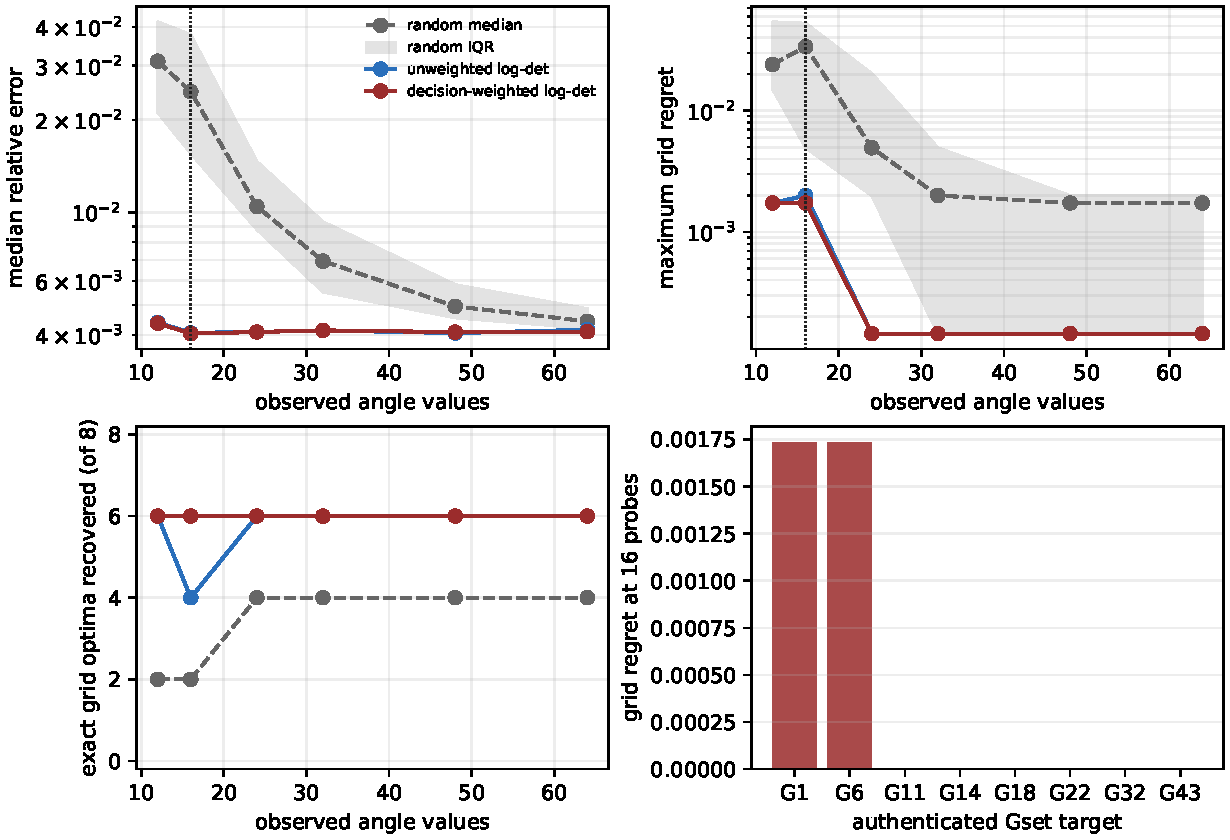
\includegraphics[width=0.94\textwidth]{code/results/decision_probe_audit.pdf}
\caption{\label{fig:decision}Probe-budget audit.  Top: surface error and grid
regret, with the random interquartile range.  Bottom left: exact optimizer
recovery.  Bottom right: targetwise regret at the predeclared 16-probe budget.
The remaining regret is concentrated on G1 and G6, which share the same
unweighted topology.}
\end{figure*}

At 24 and more probes, the selected decision weight is often zero and the two
D-optimal designs coincide.  The method is therefore most consequential in
the low-budget regime; it is not a blanket replacement for unweighted design.

Figure~\ref{fig:certificate} evaluates Theorem~\ref{thm:recovery} under five
noise levels.  All simulated errors remain below the deterministic bound, but
the bound is conservative.  The runtime panel supplies a separate negative
control: at rank 12, row-Gram learning takes a median 2.98 ms, hierarchical
actions 8.36 ms, and thin SVD 27.10 ms.  Reduced retained-operator storage does
not imply a wall-clock advantage at $120\times1024$.

\begin{figure*}[t]
\centering
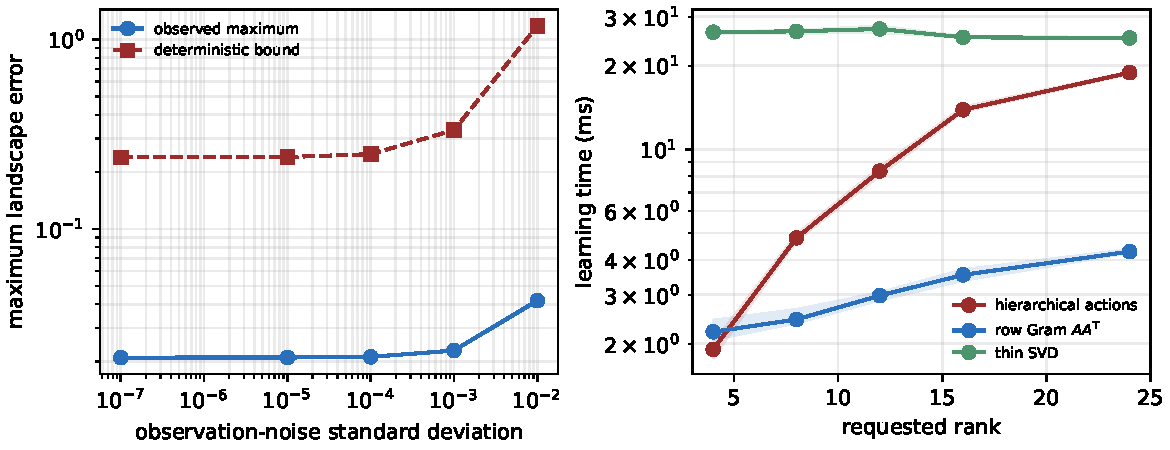
\includegraphics[width=0.86\textwidth]{code/results/certificate_runtime_audit.pdf}
\caption{\label{fig:certificate}Validity and cost.  Left: observed maximum
landscape error and the deterministic bound in Theorem~\ref{thm:recovery}.
Right: median learning time with interquartile bands over 15 repetitions; the
hierarchy construction and data-loading stages are excluded for every method.}
\end{figure*}

\section{Scope and reproducibility}

The package records source addresses and hashes, the complete calibration
grid, all probe indices, 64 random seeds, targetwise outcomes, noise draws,
operation counts, runtime repetitions, and theorem checks.  A deterministic
CPU command recreates the 120 development landscapes and eight public targets,
regenerates the displayed artifacts, and compares the scientific payload with
the locked result.

The experiment does not evaluate weighted Gset objectives, depth greater than
one, hardware noise, or global MaxCut approximation quality.  The method
improves a low-budget angle-selection decision on this corpus.  The disclosed
source and budget boundaries are part of that claim.

\bibliographystyle{apsrev4-2}
\bibliography{code/manuscript_assets/references}

\end{document}
